\documentclass[12pt,floatfix,showpacs]{revtex4-1}

\usepackage{amssymb,amsmath,amsfonts}
\usepackage{graphicx}
\usepackage{subfig}
\usepackage{epstopdf}

\newcommand{\eg}{\emph{e.g., }}
\newcommand{\ie}{\emph{i.e., }}
\newcommand{\etal}{\emph{et al.}}
\newcommand{\diff}{\ensuremath\mathrm{d}}

% remove these for final publication 
\usepackage{color} 
\newcommand{\note}[1]{\textcolor{red}{#1}}
\newcommand{\gnote}[1]{\marginpar{\scriptsize\textcolor{red}{#1}}}

\graphicspath{{./graphics/}}

% Macro to consistently format the package name:
\usepackage{xspace}
\newcommand{\eqtools}{\texttt{eqtools}\xspace}

\usepackage{siunitx}

\begin{document}

\title{\eqtools: Modular, Extensible, Open-Source, Cross-Machine Python Tools for Working with Magnetic Equilibria}

\author{M. A. Chilenski}
\email[]{markchil@mit.edu}
\affiliation{MIT Plasma Science and Fusion Center}

\author{I. C. Faust}
\affiliation{MIT Plasma Science and Fusion Center}

\author{J. R. Walk}
\affiliation{MIT Plasma Science and Fusion Center}

\date{\today}

\begin{abstract}
As experimental plasma physics research transitions to be predominantly conducted across institutions and machines, it becomes increasingly important that portable tools be developed to enable data from diverse sources to be analyzed in a consistent manner. 
This paper presents \eqtools, a modular, extensible, open-source toolkit implemented in the Python programming language for handling magnetic equilibria and associated data from tokamaks. 
\eqtools provides a single interface for working with magnetic equilibrium data, both for handling derived quantities and mapping between coordinate systems, extensible to function with data from different experiments, data formats, and magnetic reconstruction codes, replacing the diverse, non-portable solutions currently in use.  
Moreover, implementing these tools in Python removes a substantial barrier to code migration and new development in the open-source Python programming language, which presents a number of advantages.  
In this paper, we introduce the design of the \eqtools package and detail the workflow for usage and expansion to additional devices.  The implementation of a novel three-dimensional spline solution (in two spatial dimensions and in time) is also detailed.  
Finally, benchmarking for accuracy and speed against existing tools are detailed. Wider deployment of these tools will enable efficient sharing of data and software between institutions and machines as well as self-consistent analysis of the shared data.
\end{abstract}
\gnote{other PACs numbers?}

\pacs{52.55.Fa}

\maketitle

%%%%%%%%%%%%%%%%%%%%%%%%%%%%%%%%%%%%%%%%%%%%%%%%%%%%%%%%%%%%

\section{Introduction}\label{sec:intro}

The basic computational tasks associated with magnetic equilibrium reconstructions -- namely, the handling of derived quantities (\eg calculated plasma current, safety-factor profiles) and the mapping between real-space and flux coordinate systems for experimental data -- are universal among tokamak experiments.  
Despite this commonality, experiments typically utilize in-house solutions developed for the particulars of that experiment's data storage and usage.  
This ad-hoc development of base-level functionality inhibits the mobility of higher-level codes to other devices (as the code may require substantial modification to address the particulars of the new data storage design).  
Moreover, such development is often quite static, such that the implementation is difficult to extend to new data formats (for example, to handle both a primary MDSplus-based data storage system \cite{MDSplus} and the \emph{eqdsk} storage files produced directly by the EFIT reconstruction code \cite{Lao1985}), necessitating parallel workflows for functionally identical tasks depending on the data source.  
Best design practices call for the vagaries of data source and storage implementation to be placed in the back end, presenting a consistent, straightforward interface common between machines and code implementations to the research scientist.

The new \eqtools package provides a modular, extensible, cross-machine toolkit developed in the Python programming language for handling magnetic equilibrium data.  
The \eqtools package provides a consistent and straightforward interface to the researcher for both coordinate mapping routines (historically handled in separate standalone routines) and access to derived quantities (often handled with manual hooks into data storage).  
Moreover, \eqtools is constructed with a modular, object-oriented design, such that the package is easily extensible to handle data from different experiments and reconstruction codes, giving the researcher a single unified interface for data from any machine or code.  
The implementation of reconstructed-equilibrium handling in the Python language removes a substantial barrier to the adoption of Python as a day-to-day analysis language for tokamak research, which offers numerous advantages in ease of use, computational speed, user/developer base, and free and open-source implementations compared to current common working languages for fusion research.  The \eqtools package is open-source and licensed under the GNU General Public License \cite{GPL}, and distributed via GitHub \cite{eqtools_git,eqtools_readthedocs}.

This paper details the design and implementation of \eqtools, particularly the paradigm for extension to new machines (section \ref{sec:design}), describes the basic algorithms used to convert between coordinate systems (section \ref{sec:algo}), describes the implementation of a trivariate spline method for improved interpolation in the time dimension (section \ref{sec:trispline}), and presents runtime and accuracy benchmarks against the current IDL implementation at Alcator C-Mod (section \ref{sec:benchmark}).

\section{Package Design and Use}\label{sec:design}

The \eqtools package is designed to present a consistent, human-readable interface to the user for both data handling of derived quantities and mapping routines between coordinate systems, all contained within a single persistent object (herein referenced in code snippets as \verb|eq|).
For example, consider how the poloidal flux on-axis would be accessed using the current system on Alcator C-Mod using the MDSobjects \cite{MDSobjects} Python interface:
\begin{verbatim}
import MDSplus
t = MDSplus.Tree('analysis', shotnum)
n = t.getNode('efit.results.a_eqdsk:simagx')
psi0 = n.data()
\end{verbatim}
And compare to the approach to access the same data using \eqtools:
\begin{verbatim}
import eqtools
eq = eqtools.CModEFITTree(shotnum)
psi0 = eq.getFluxAxis()
\end{verbatim}
Notice that the \eqtools approach requires fewer lines and that the cryptic six letter EFIT tag name ``simagx'' is replaced with the more descriptive ``getFluxAxis.''
%For example, accessing the calculated value for the poloidal flux on-axis, $\psi_0$, is simply \verb|eq.getFluxAxis()| -- this replaces arrangements that may involve manual hooks into the data system (as is the case at Alcator C-Mod) and interaction with non-intuitive internal variable names (as is the case with EFIT outputs\gnote{too harsh?}\gnote{Perhaps we could emphasize this with code snippets of the old way?}).  
Similarly, mapping routines are handled internally in the \verb|eq| object -- mapping from the machine RZ grid to normalized poloidal flux, for example, is simply \verb|eq.rz2psinorm(R,Z,t,...)|.  
One notable consequence of this is that intermediate spline calculations for the mapping routines are stored in the persistent object -- compared to typical standalone mapping routines (which must start from scratch for each function call) this allows substantial speed gains for subsequent mapping calculations with the same equilibrium object, as is illustrated in section~\ref{sec:benchmark}.

The \eqtools package is structured such that the user-facing methods (for data access and coordinate mapping) are consistent for different machines or reconstruction codes, and moreover adding support for new machines or codes requires minimal new code.  
The package inheritance structure is depicted in figure \ref{fig:flowchart}.  
The base level of the inheritance structure (shown in blue in figure \ref{fig:flowchart}) provides the abstract class \verb|Equilibrium| -- this defines the skeleton structure for the data system (ensuring that child classes use a consistent format) and defines the mapping routines, which are inherited and used by each child class.  
The methods therein are sufficiently general to be used by any grid-based equilibrium reconstruction.

\begin{figure}[p]
 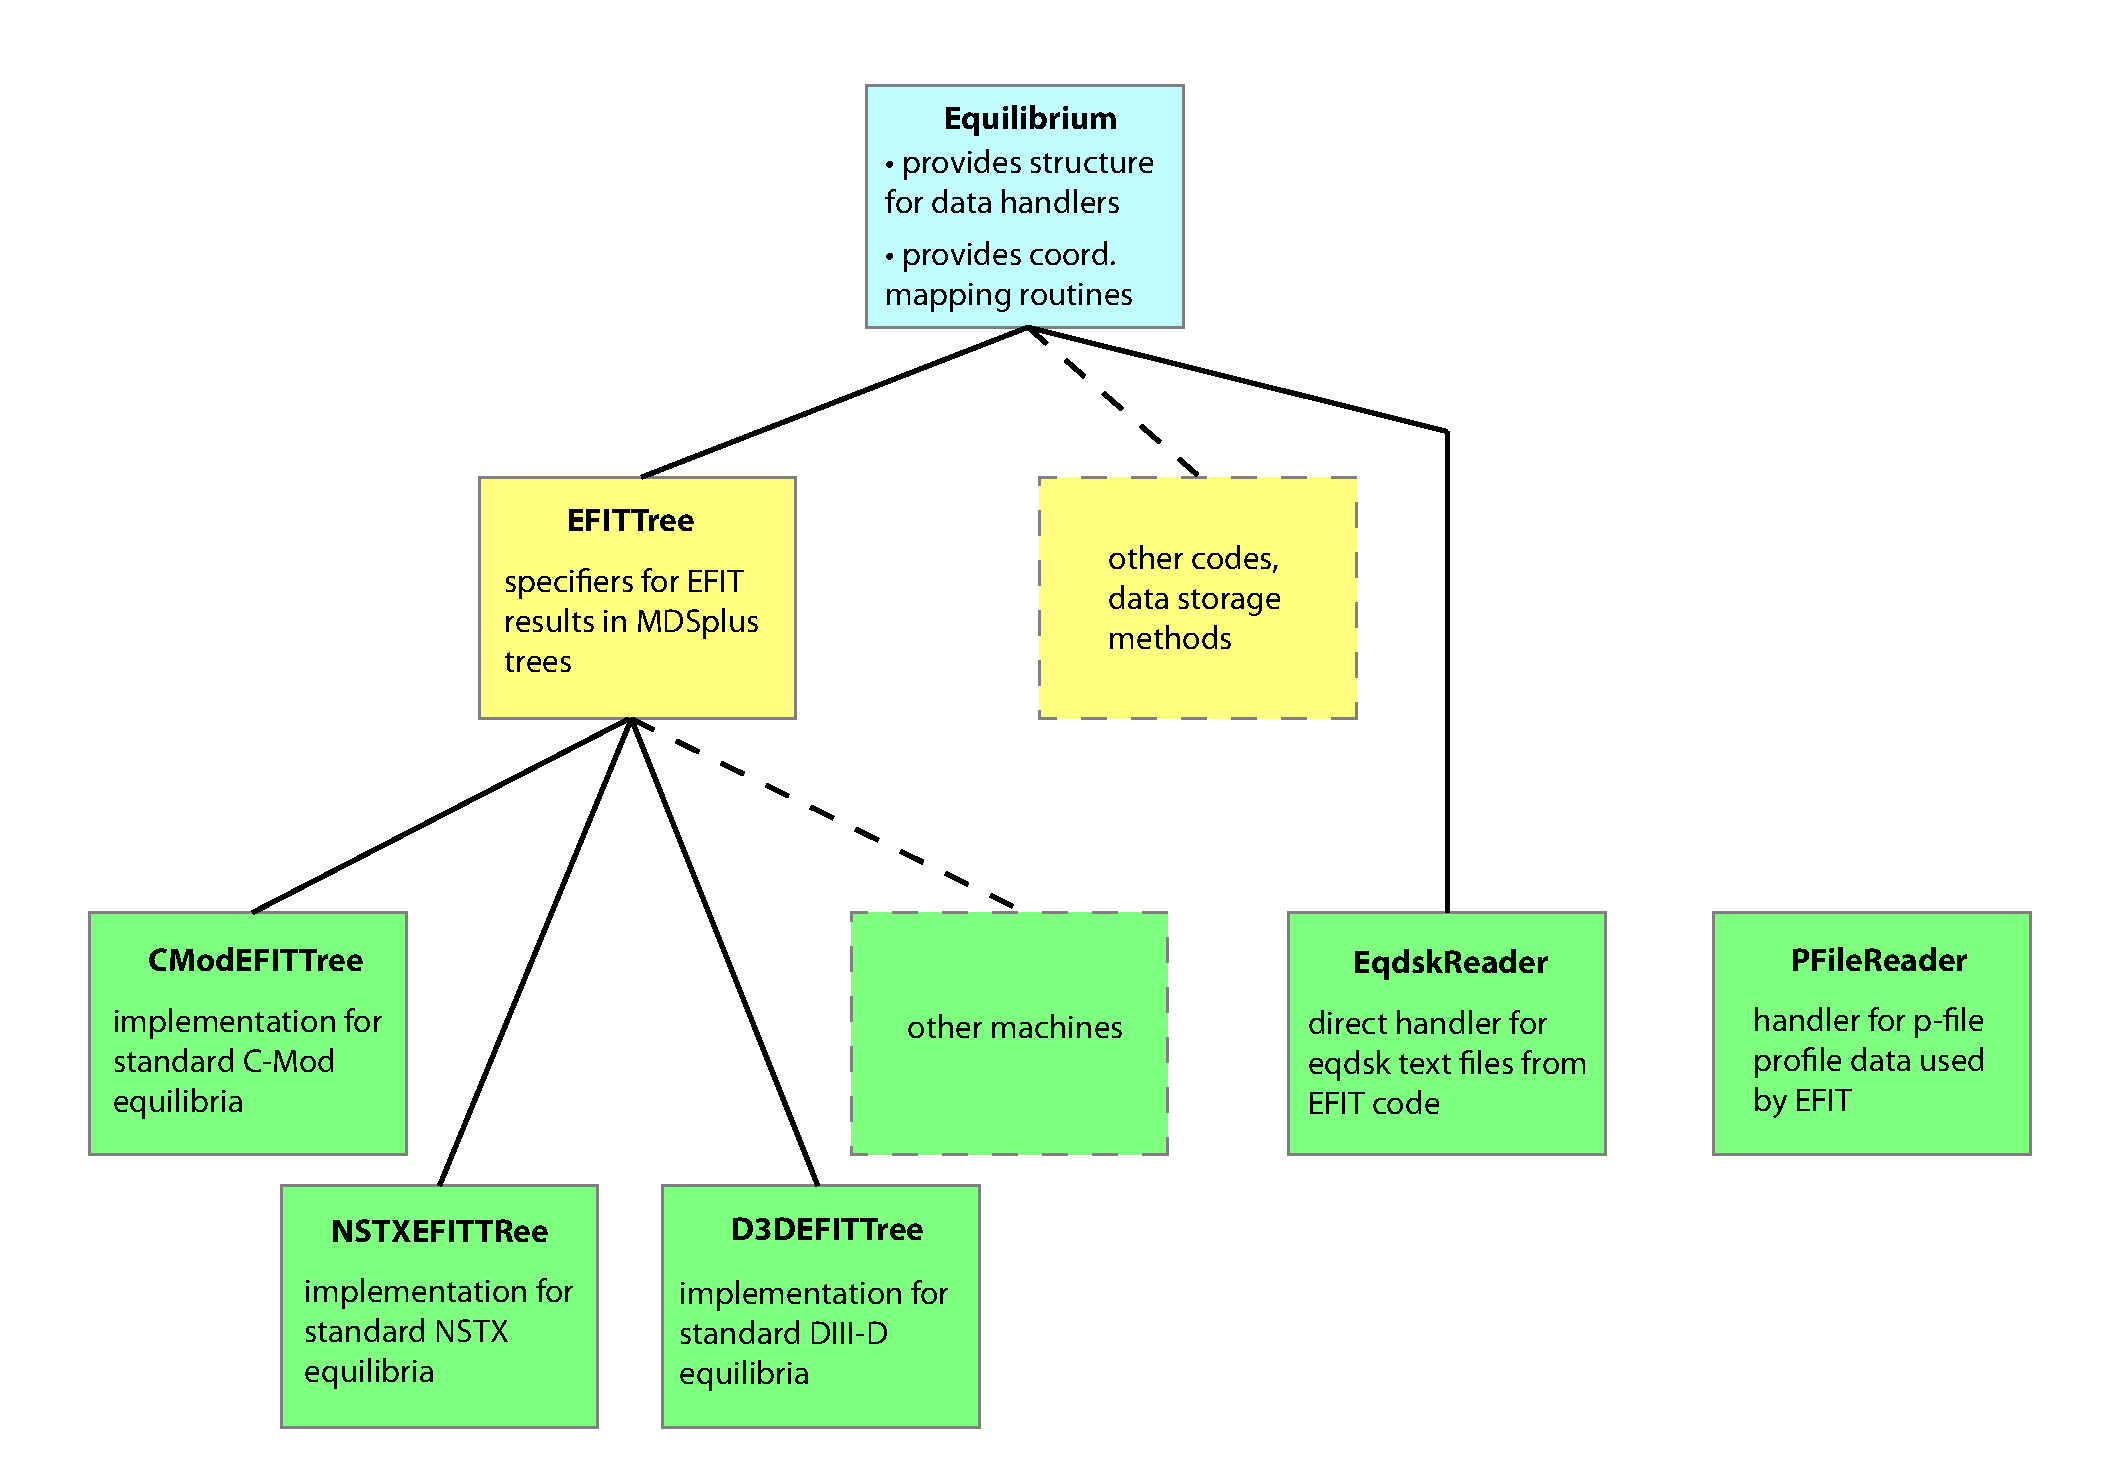
\includegraphics[width=\textwidth]{graphics/flowchart.pdf}
 \caption{Inheritance schematic for the \eqtools package.  The base abstract class (blue) provides a skeleton structure for the derived-data handlers, as well as providing the complete set of coordinate-mapping routines.  Intermediate abstract classes (yellow) prescribe the handling for data storage systems and codes -- at present the relatively-ubiquitous EFIT reconstruction stored in MDSplus tree structures is provided.  User-facing classes (green) handle the details of machine-specific implementations.  Dashed lines denote classes that have not yet been implemented, but which can be introduced into the package in a straightforward manner due to its modular construction.  The user interface is consistent, as it is provided by the parent classes -- code migration between machines requires only changing which child class is called for the reconstruction.  The \texttt{EqdskReader} class, which directly handles \emph{eqdsk} text files from EFIT, inherits directly from the base class as it is sufficiently unique to not warrant an intermediate abstract class.  \note{add filewriter?}}
 \label{fig:flowchart}
\end{figure}

An intermediate inheritance level (shown in yellow in figure \ref{fig:flowchart}) provides more specific methodology (while still maintaining cross-machine generality) -- for example, the \verb|EFITTree| class provides methods for EFIT reconstructions stored in MDSplus tree structures (as is used on C-Mod, NSTX, and DIII-D\gnote{cites?}).  
This minimizes the need for repeated code in machine-specific versions of common code implementations.  
The user-facing inheritance level (shown in green in figure \ref{fig:flowchart}) finalizes the specific details of implementation for a given reconstruction code, data-storage methodology, and machine implementation (\eg \verb|CModEFITTree|, \verb|NSTXEFITTree|, \verb|D3DEFITTree|).  
These user-facing implementations typically require relatively little code (on the order of 100 lines in the case of \verb|CModEFITTree| and \verb|NSTXEFITTree|), and extension modules to the code can be quickly developed in most cases.

In addition to the already-developed modules inheriting \verb|EFITTree|, the code currently contains the \verb|EqdskReader| module, which directly interfaces with the \emph{eqdsk} text files (specifically, the ``g-file'' and ``a-file'' containers, which store equilibrium and scalar derived quantities, respectively) generated by EFIT.\gnote{cite?}  
This allows a single unified interface for both the tree-based and portable text-file data storage common to US experiments.\gnote{expand?  other countries?}  
Due to the unique structure of the code necessary to read text-file data (which is done directly in \verb|EqdskReader|), \verb|EqdskReader| directly inherits mapping routines and skeletal structure from \verb|Equilibrium|, without an intermediate stage; however, as new text-file-based storage methods are implemented in \eqtools sufficient commonality may be found to necessitate the creation of a intermediate abstraction level for generalized text-file storage systems in subsequent versions of the \eqtools package.

In addition to the \verb|EqdskReader| module, which handles equilibrium and derived-quantity data from g- and a-file outputs from EFIT, the \eqtools package provides a \verb|PFileReader| object to handle plasma-profile data from the ``p-files'' associated with EFIT.  
While this does not require access to the reconstructed equilibrium (and thus is separate from the \verb|Equilibrium| inheritance structure) profile data is commonly paired with the reconstructed equilibrium -- as such, the \eqtools package provides a built-in methodology to handle the additional data.  
The \eqtools package also contains a package-level method, \verb|filewriter|\gnote{check naming!} to produce g-files from classes in the \verb|Equilibrium| inheritance tree, allowing easy generation of portable datasets from the main data-storage method.\gnote{reword?}

\section{Details of the coordinate mapping routines}\label{sec:algo}
One of the strengths of \eqtools is its support for conversions between the majority of coordinate systems in common use:
\eqtools supports transformations between a wide variety of coordinates including real space $(R, Z)$ coordinates, mapped outboard midplane major radius $R_{\text{mid}}$, normalized minor radius $r/a$, unnormalized poloidal flux $\psi$, normalized poloidal flux $\psi_{\text{n}}$, normalized toroidal flux $\phi_{\text{n}}$, normalized flux surface volume $V_{\text{n}}$ and the square roots of these quantities.\gnote{John, not sure what more breakdown you want here. Please clarify your comments.}

The basic transformation is to map a given point $(R, Z)$ at a given time $t$ to the poloidal flux $\psi$ at that location as computed with the magnetic reconstruction code.
The default implementation uses a nearest-neighbor interpolation in time: the code first retrieves the flux reconstruction at the time closest to $t$, then a bivariate interpolating spline \cite{dierckxBook,scipy} is used to map from $(R, Z)$ to $\psi$.
The bivariate spline coefficients from each time are stored in memory as they are computed in order to speed up subsequent calculations at that time slice.
A more advanced method using a tricubic interpolating spline to interpolate smoothly in space \emph{and} time is described in section~\ref{sec:trispline}.

Once the coordinate has been mapped to $\psi$, subsequent calculations are simpler.
Normalized poloidal flux is defined as
\begin{gather}
	\psi_{n} = \frac{\psi - \psi_{0}}{\psi_{a} - \psi_{0}},
\end{gather}
where $\psi_{0}$ is the poloidal flux at the magnetic axis and $\psi_{a}$ is the poloidal flux at the boundary.
To ensure self-consistency, the default behavior is to use nearest-neighbor interpolation to get the values of $\psi_{0}$ and $\psi_{a}$ at the desired time.
When a tricubic spline is used to map from $(R, Z)$ to $\psi$ a cubic spline is used to interpolate these values in time.

Normalized toroidal flux is defined in terms of normalized poloidal flux as
\begin{gather}
	\phi(\psi) = \int_{\psi_{0}}^{\psi} q(\psi')\,\diff\psi'\label{eq:phipsi}\\
	\phi_{\text{n}} = \frac{\phi}{\phi_{a}},
\end{gather}
where $q = \diff\phi/\diff\psi$ is the safety factor profile (typically computed when EFIT is run) and $\phi_{a}=\int_{\psi_{0}}^{\psi_{a}}q(\psi')\,\diff\psi'$ is the toroidal flux at the last closed flux surface.
The integral in (\ref{eq:phipsi}) is numerically evaluated using the trapezoid rule.

The normalized flux surface volume is defined as
\begin{gather}
	V_{\text{n}}(\psi) = \frac{V(\psi)}{V_{a}},
\end{gather}
where $V_{\psi}$ is the volume enclosed by the (closed) flux surface with flux $\psi$ and $V_{a}$ is the volume enclosed by the last closed flux surface.
In the case of Alcator C-Mod, the flux surface volume $V(\psi)$ is computed automatically when EFIT is run, but it would be straightforward to override the \verb|getFluxVol| method of the \verb|Equilibrium| class to compute this from the $\psi(R, Z)$ grid when this quantity is not already available in the tree.
Mapping from $\psi_{\text{n}}$ to $R_{\text{mid}}$ is accomplished by forming a dense radial grid of $R$ points that go from the magnetic axis to the edge of the grid the flux is reconstructed on, finding the vertical location of the magnetic axis at the desired time(s) (called $Z_{0}$), then converting the resulting $(R, Z_{0})$ points to $\psi_{\text{n}}$ with the routines described above.
This one-to-one mapping between $R_{\text{mid}}$ and $\psi_{\text{n}}$ is then interpolated to give the desired conversion from $\psi_{\text{n}}$ to $R_{\text{mid}}$.

By default, $r/a$ is defined in terms of $R_{\text{mid}}$ as
\begin{gather}
	r/a = \frac{R_{\text{mid}} - R_{0}}{R_{a} - R_{0}},
\end{gather}
where $R_{0}$ is the major radius of the magnetic axis and $R_{a}$ is the outboard midplane major radius of the last closed flux surface.
Since other definitions of $r/a$ are preferred when the Shafranov shift is high, the specific definition of $r/a$ can be changed simply by overriding the methods \verb|_rmid2roa| and \verb|_roa2rmid| in the \verb|Equilibrium| class.
Variants on these basic routines are then used to map between other pairs of coordinates.

\section{Tri-Spline Implementation}\label{sec:trispline}

\begin{figure}[ht]
 \includegraphics[width=\textwidth]{graphics/tspline_merge.eps}
 \caption{Flux surface reconstruction in time of a Alcator C-Mod discharge using nearest-neighbor time interpolation (a) and a tricubic spline interpolation (b). Aliasing behavior removed by the use of a spline in the time-dimension. }
 \label{fig:tspline}
\end{figure}

Time-dependent interpolation poses a difficult problem with respect to the instantaneous nature of most equilibrium reconstructions. 
Usually coordinates are often determined via interpolation using the closest equilibrium in time.
When the sampling rate of equilibria is lower than the desired coordinate sampling rate, this can induce aliasing behaviors (as can be seen in \ref{fig:tspline}). 
The aliasing-induced discontinuities pose an issue for long timescale behaviors of coordinates.  
When the set of equilibria achieves the Nyquist frequency for variations of interest, an additional interpolation in time can accurately remove aliasing errors induced by this timebase mismatch. 
The additional temporal dimension requires the use of higher dimensional interpolators, for which a fast tricubic interpolation scheme was developed. 

The additional time dimension and subsequent higher-dimensionality increases the evaluation time of the mapping routines. 
A tricubic interpolating spline \cite{Lekien2005} is used to evaluate the three-dimensional flux grid. 
The time dimension is assumed to be like a rectilinear spatial dimension which allows for the use of developed optimized matrix methods for extracting the necessary spline coefficients. 
The higher dimensionality of the problem scales the necessary computational time due to the increased necessary information ($\times64$ increase in matrix computation). 
Other non-three-dimensional parameters also require further computation due to the inherent complication of increasing the number of dimensions. 
Use of persistence of the coefficients allows for similar computational times to previous equilibrium mappings when subject to calculations in the same `voxel', the overall computation is slower when compared to lower-dimensional mapping.

Significant time savings can be recovered for tricubic interpolation computation when the data grid is regular, which is often the case for sets of magnetic equilibria. 
Recovering the spline coefficients requires the calculation of a number of derivatives in each dimension, which for a regular grid can be achieved with finite difference matrix $\boldsymbol{B}$. 
The new \emph{a priori} inclusion of $\boldsymbol{B}$ in the spline calculation matrix $\boldsymbol{A_{inv}}$ removes the necessary derivative generation and reduces total computation by half (denoted $\boldsymbol{A_{inv}^*}$). 
This calculation requires a collection of the nearest $4\times4\times4$ grid of points to the coordinates of interest $\boldsymbol{x}$ to extract spline coefficients $\boldsymbol{y}$.

\begin{equation}
\boldsymbol{y} = \boldsymbol{A_{inv}} ( \boldsymbol{B} \boldsymbol{x}) = \boldsymbol{A_{inv}^*}\boldsymbol{x}
\end{equation}
Where,
\begin{equation}
\boldsymbol{A_{inv}^*} = \boldsymbol{A_{inv}}\boldsymbol{B} 
\end{equation}

The code for the tricubic spline interpolation was written in C and was integrated into Python using F2PY \cite{Peterson2009} package. 
Other programming languages and codes with sufficient C APIs can access the optimized trispline code for use outside of magnetic reconstructions, and is well contained in accepting 3 dimensional data for analysis.

\section{Benchmarking}\label{sec:benchmark}
\eqtools has been benchmarked against the existing, thoroughly-tested IDL routines presently in use for handling coordinate mapping at Alcator C-Mod.
Figure~\ref{fig:rz2psi_diff} shows the discrepancy between IDL and \eqtools for the conversion of $(R, Z)$ to $\psi$.
The differences are small (of order \num{e-4}), and are consistent with the fact that Python defaults to double precision whereas IDL defaults to single precision.
\begin{figure}
	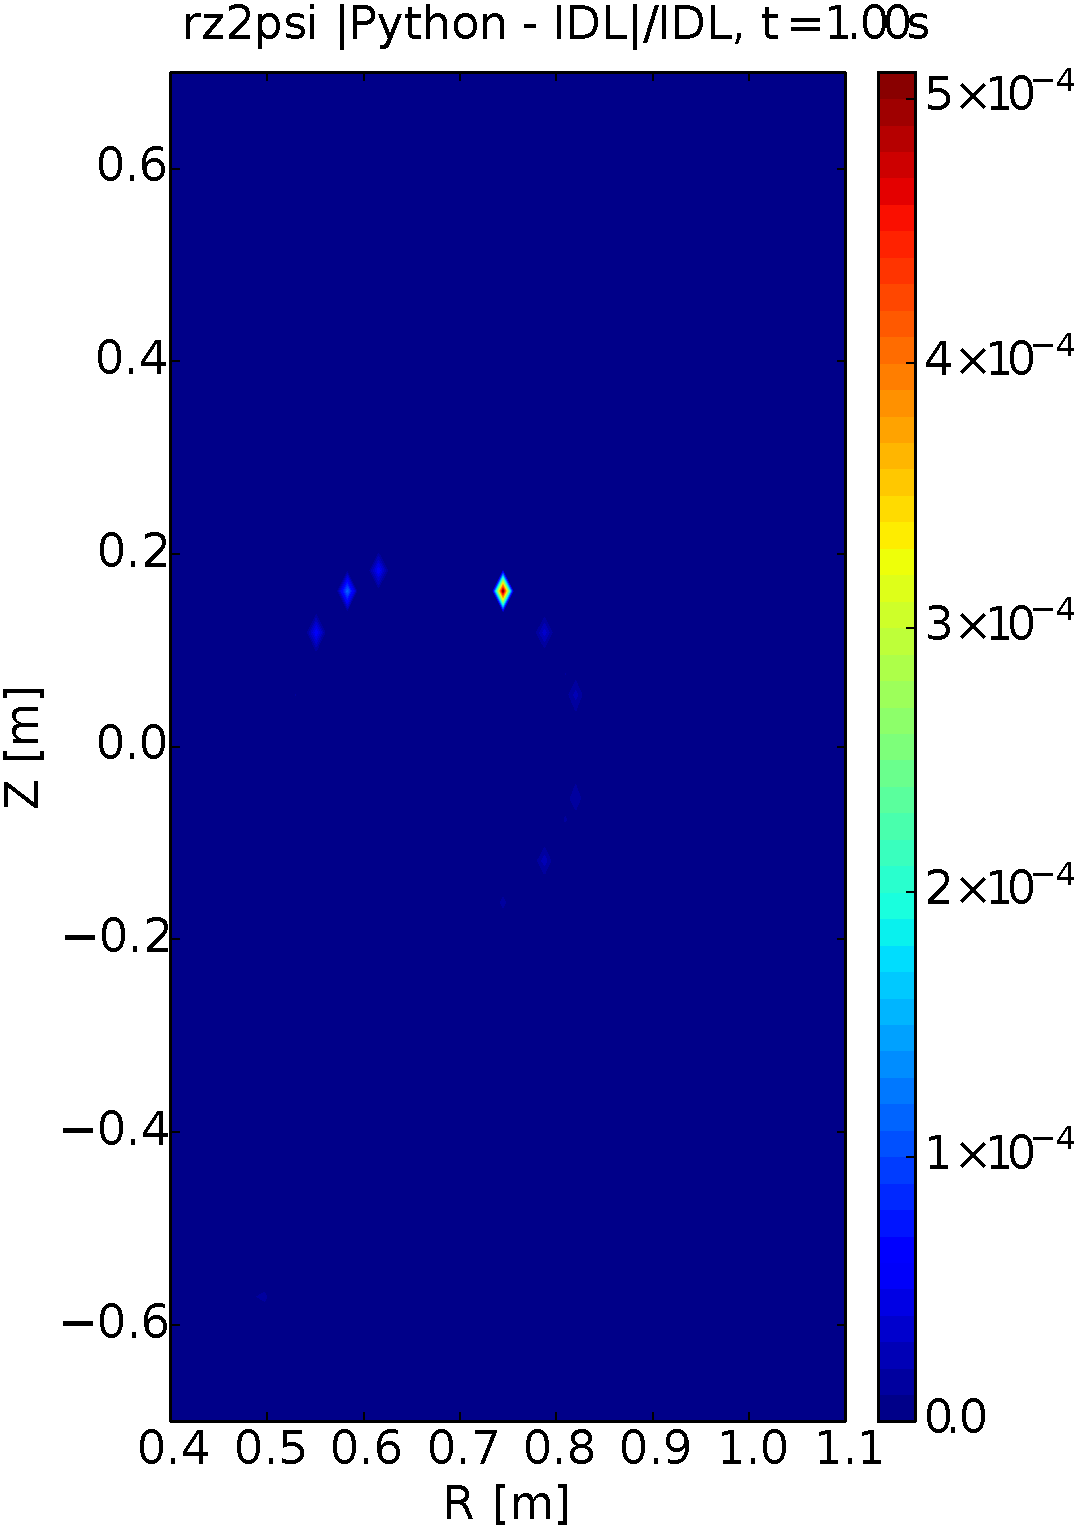
\includegraphics[width=0.5\textwidth]{graphics/rz2psi}
	\caption{Relative difference between calculations of a mapping between the RZ grid and poloidal flux for the \eqtools and the current IDL implementation of the mapping routine for an example Alcator C-Mod reconstructed equilibrium.  Relative differences of order \num{e-4} are typical, and are consistent with the different default precisions of IDL versus Python.}
	\label{fig:rz2psi_diff}
\end{figure}
Timing tests were conducted by converting a $66\times66$ element $(R, Z)$ grid (double the density of the grid EFIT provides the flux on) into each of the coordinates supported.
This conversion was performed at each of the 90 time slices output by EFIT and nearest-neighbor temporal interpolation was used.
The conversion was performed twice with the same \verb|Equilibrium| object in \eqtools in order to assess the time savings from storing the spline coefficients.
The test was repeated 100 times, and the mean execution time to convert the $(R, Z)$ grid at each time slice is given in Table~\ref{tab:benchmarkingtests}.
\begin{table}
	\caption{Mean execution times in milliseconds}
	\label{tab:benchmarkingtests}
	\begin{tabular}{lS[table-format=2.1]S[table-format=2.1]S[table-format=1.1]}
		\hline
		Conversion & {IDL} & \multicolumn{2}{c}{\eqtools}\\
		\cline{3-4}
		 & & {first run} & {second run}\\
		\hline
		$(R, Z)\to\psi$ & 11.7 & 2.5 & 1.9\\
		$(R, Z)\to\psi_{\text{n}}$ & 21.8 & 2.0 & 2.0\\
		$(R, Z)\to\phi_{\text{n}}$ & 30.2 & 3.1 & 2.3\\
		$(R, Z)\to V_{\text{n}}$ & 28.0 & 3.0 & 2.3\\
		$(R, Z)\to R_{\text{mid}}$ & 36.1 & 12.1 & 2.4\\
		\hline
	\end{tabular}
\end{table}
\eqtools is faster than the IDL-based routines by as much as a factor of ten even on the first run.
This improvement is from a combination of the switch to Python and the fact that \eqtools stores the equilibrium data in a persistent object instead of having to fetch it from the MDSplus tree for each call.
Subsequent runs with the same \verb|Equilibrium| object are faster, particularly for the conversion to $R_{\text{mid}}$, which has considerable overhead on the first call.

\section{Summary}\label{sec:summary}

The \eqtools package provides a modular, extensible framework for handling the basic tasks associated with magnetic equilibrium reconstructions for tokamaks -- namely, accessing derived quantities and mapping between real-space and flux coordinate systems for experimental data.
This package, developed in the open-source Python programming language and freely available from Github \cite{eqtools_git,*eqtools_readthedocs}, presents a consistent, user-friendly interface independent of data source or storage method, replacing machine- and storage-specific methods which are often nonintuitive to use and which often use a static code structure that can be difficult to extend for experimental data from multiple machines, storage methods, or reconstruction codes.
Moreover, the \eqtools package is designed with a modular, object-oriented construction, such that the package is easily extended to include new experiments, reconstruction codes, and data storage methods (in the current distribution version, EFIT reconstructions \cite{Lao1985} in MDSplus-based data storage from NSTX, C-Mod, and DIII-D are implemented, along with a class to read the portable \emph{eqdsk} datafile).  

The package includes a complete set of mapping routines between real-space machine coordinates (that is, the $RZ$ grid defined for the reconstruction), midplane-mapped real-space coordinates (major radius and normalized minor radius), and flux-space coordinate systems (normalized poloidal and toroidal flux and normalized flux surface volume), as well as their square roots -- in short, the coordinate systems customarily used in a broad variety of analysis applications are supported within a single unified user interface.  
In addition to the standard bivariate analysis mapping the $R$ and $Z$ coordinate with nearest-neighbor interpolation in time (as is used in the mapping routines presently used on C-Mod), \eqtools allows for a trivariate spline providing smooth interpolation along the time axis as well.  
This allows the user to optionally trade computational time for a substantially more accurate treatment of the time variation in cases where experimental data are sampled at times significantly different from the reconstruction timebase.

The mapping routines in \eqtools have been thoroughly benchmarked against the existing IDL implementations used at Alcator C-Mod.  
Mapping results from \eqtools are consistent with the previous IDL results to within numerical error (arising from double-precision calculations in Python compared to the default single precision used in IDL).
Initial runs of the \eqtools mapping routines are a factor of three to ten faster than the previous IDL implementation.
Moreover, as the persistent \verb|Equilibrium| object stores intermediate calculations in the mapping routines, subsequent calculations with the same shot show additional speed improvements compared to the IDL implementation.

The development of \eqtools clears a substantial hurdle to the adoption of Python as a standard data analysis language for tokamak research, the use of which offers numerous advantages in terms of development base and support, computational speed, ease of adoption, and cost over other languages in common use at present.
Additionally, \eqtools allows for substantially more straightforward implementation of cross-machine analysis tools, a significant benefit in light of increasing emphasis on modeling and cross-machine collaboration in fusion research.

%%%%%%%%%%%%%%%%%%%%%%%%%%%%%%%%%%%%%%%%%%%%%%%%%%%%%%%%%%%%

\begin{acknowledgements}
The authors would like to acknowledge their thanks for the work S.~Wolfe performed in writing the original IDL coordinate mapping routines for Alcator C-Mod.

This material is based upon work conducted using the Alcator C-Mod tokamak, a DOE Office of Science user facility.
This material is based upon work supported by the U.S.\ Department of Energy, Office of Science, Office of Fusion Energy Sciences under Award Number DE-FC02-99ER54512.
This material is based upon work supported in part by the U.S.\ Department of Energy Office of Science Graduate Research Fellowship Program (DOE SCGF), made possible in part by the American Recovery and Reinvestment Act of 2009, administered by ORISE-ORAU under contract number DE-AC05-06OR23100.

\end{acknowledgements}


\bibliographystyle{aipnum4-1}
\bibliography{eqtools_paper}

\end{document}
